% Tikz File 'boutrophedon_transition_types.tex'
\documentclass{standalone}
\usepackage{tikz}

\usetikzlibrary{shadows.blur}
\usetikzlibrary{shapes.symbols}

%==============================================================================%
% TiKz Templates
\tikzset{% 
	box/.style={very thick,blur shadow={shadow blur steps=5},fill=white}
}
\tikzset{% 
	covered_area/.style={fill=green,opacity=0.4}
}
%==============================================================================%

\begin{document}
	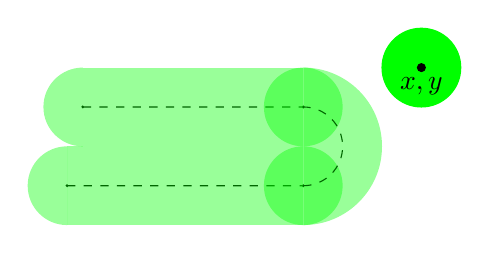
\begin{tikzpicture}[scale=1]
		\coordinate (p1) at ([xshift= 0.5cm,yshift=0.5cm]0,0);
		\coordinate (p2) at ([xshift=-0.5cm,yshift=0.5cm]4,0);
		\coordinate (p3) at ([xshift= 0.7cm,yshift=1.5cm]0,0);
		\coordinate (p4) at ([xshift=-0.5cm,yshift=1.5cm]4,0);

		%\draw [box] (p1)--(p2)--(p3)--(p4)--cycle;

		\draw [fill,color=green] (5,2) circle [radius=0.5cm];
		\draw [fill] (5,2) circle [radius=0.05cm] node[below]{$x,y$};

		%First line
		\draw [dashed] (p1) circle [radius=0.01cm]--(p2) circle [radius=0.01cm];
		\fill [covered_area] ([yshift=-0.5cm]p1) rectangle ([yshift=0.5cm]p2);
		\fill [covered_area] ([yshift=0.5cm]p1) arc (90:270:0.5cm);
		\fill [covered_area] ([yshift=0.5cm]p2) arc (90:-90:0.5cm);

		%Second line
		\draw [dashed] (p3) circle [radius=0.01cm]--(p4) circle [radius=0.01cm];
		\fill [covered_area] ([yshift=-0.5cm]p3) rectangle ([yshift=0.5cm]p4);
		\fill [covered_area] ([yshift=0.5cm]p3) arc (90:270:0.5cm);
		\fill [covered_area] ([yshift=0.5cm]p4) arc (90:-90:0.5cm);

		%Transition line
		\draw [dashed] (p2) arc (-90:90:0.5cm);
		\fill [covered_area] ([yshift=-0.5cm]p2) arc (-90:90:1.0cm);
		\fill [covered_area] ([yshift=0.5cm]p2) arc (90:270:0.5cm);
		\fill [covered_area] ([yshift=0.5cm]p4) arc (90:270:0.5cm);

	\end{tikzpicture}
\end{document}